\section{Probabilistic demand forecasting}\label{sec:forecasting}

Capacity planning needs a \emph{distribution} of tomorrow's demand at the zone--category level, and the joint behaviour of the 260 series.
This section builds the marginal forecasts; \cref{sec:scenarios} turns them into joint scenarios.

\subsection{Protocol}
We use a rolling-origin backtest.
Every day $\tau$ we forecast $h=1,\dots,7$ days ahead for all 260 series, using only information available at the end of day $\tau$.
Models are retrained quarterly on an expanding window, on six dates from June 2025 to September 2026; no training target lies after the retraining date.
The origins are split in two:
\begin{itemize}
  \item a \textbf{validation} period (June--September 2025, including Prime Day 2025), used for every modelling decision;
  \item a \textbf{test year} (targets from 1 October 2025 to 30 September 2026), never used for design decisions.
\end{itemize}
Accuracy is measured by:
\begin{itemize}
  \item the weighted MAPE (wMAPE) of the median, $\sum|y-\hat y_{0.5}|/\sum y$, and its bias;
  \item the scaled quantile loss (SQL) over seven levels $a\in\{0.05,0.1,0.25,0.5,0.75,0.9,0.95\}$, $\mathrm{SQL}=\frac{1}{7}\sum_a \sum \rho_a(y-\hat y_a)/\sum y$, where $\rho_a$ is the pinball loss. Twice the SQL approximates the scaled CRPS, a strictly proper score \citep{gneiting2007};
  \item the empirical coverage and width of the central 80\% and 90\% intervals.
\end{itemize}

\subsection{Models}
\begin{itemize}
  \item \textbf{Seasonal naive}: $\hat y_{\tau+h}=y_{\tau+h-7}$. Its quantiles come from the trailing 8-week empirical distribution of multiplicative errors, per series and horizon.
  \item \textbf{LightGBM-Q} \citep{ke2017}: one \emph{global} gradient-boosted model per quantile level, trained with the pinball loss on all series and horizons jointly (1.7 million rows per retraining). The target is $y_{\tau+h}/\bar y_\tau$, normalised by the trailing 28-day mean, which makes the problem scale-free: one model serves Soria and Madrid. There are 43 features (\cref{app:features}): lags, momentum at the series, regional and national level, the calendar of the target day, announced promotions, weather forecasts, and \emph{event-aligned} year-over-year ratios. The latter compare with last year's Black Friday or Prime Day at the same offset, rather than with the same calendar date. Quantile crossing is removed by monotone rearrangement \citep{chernozhukov2010}.
  \item \textbf{Chronos-Bolt} \citep{ansari2024}: a pretrained time-series foundation model (small, 48M parameters, and base, 205M), applied \emph{zero-shot} to the raw history (context up to 2048 days) without covariates. It outputs the 0.1--0.9 quantiles; the outer levels are extrapolated in normal-score space. Inference over all 487 origins and 260 series takes under three minutes on one consumer GPU (RTX 5070 Ti).
  \item \textbf{Conformal calibration (+CP).} Every forecaster can be recalibrated by rolling split-conformal prediction, separately for each quantile level $a$, horizon $h$ and category $k$. The corrected quantile is
  \[ \tilde y_a = \hat y_a + \hat y_{0.5}\cdot \mathrm{Quantile}_a\Big\{ \tfrac{y_{o'+h}-\hat y_{a,o'}}{\hat y_{0.5,o'}} \Big\}, \]
  where the scores come from the last 56 origins $o'$ whose outcome is already known at the current origin. This is the per-level form of conformalised quantile regression \citep{romano2019}. A rolling window adapts to drift, in the spirit of adaptive conformal inference \citep{gibbs2021}.
  \item \textbf{Oracle}: Monte Carlo quantiles of the true conditional distribution (\cref{sec:dgp}). The oracle knows the latent states at the origin and the realised weather; it marks the irreducible noise floor.
\end{itemize}

\paragraph{Model selection on the validation period.}
Two choices were made on validation data only.
\begin{itemize}
  \item Replacing the day-of-year Fourier terms by the month reduced the mean validation wMAPE from 12.61\% to 12.38\%. With fine-grained seasonal encodings and only two past years, the trees memorise dates instead of learning event effects.
  \item The event-aligned year-over-year features were adopted. Larger models (1500 rounds, 127--255 leaves) did not help.
\end{itemize}

\subsection{Results}
\begin{table}[t]
\centering\small
\caption{Forecast accuracy on the test year (260 series, 365 origins, all quantities aggregated over series). SQL: scaled quantile loss; width: mean 80\% interval width relative to demand; CP: conformal calibration.}\label{tab:forecast}
\begin{tabular}{@{}lrrrrrrrr@{}}\toprule
 & \multicolumn{2}{c}{wMAPE (\%)} & Bias (\%) & \multicolumn{2}{c}{SQL (\%)} & \multicolumn{2}{c}{Coverage (\%)} & Width \\
\cmidrule(lr){2-3}\cmidrule(lr){4-4}\cmidrule(lr){5-6}\cmidrule(lr){7-8}\cmidrule(lr){9-9}
Method & $h{=}1$ & $h{=}7$ & $h{=}1$ & $h{=}1$ & $h{=}7$ & 80\% & 90\% & 80\% \\ \midrule
Seasonal naive & 24.3 & 24.6 & +0.4 & 8.02 & 8.20 & 77.6 & 86.6 & 79.8 \\
Seasonal naive + CP & 24.6 & 25.1 & +0.7 & 8.32 & 8.81 & 76.8 & 86.4 & 89.2 \\
\midrule
Chronos-Bolt-S & 15.5 & 16.9 & -2.3 & 4.80 & 5.30 & 79.3 & 88.0 & 45.6 \\
Chronos-Bolt-S + CP & 15.5 & 17.2 & -1.3 & 4.84 & 5.47 & 79.5 & 89.4 & 46.8 \\
Chronos-Bolt-B & 15.4 & 16.8 & -1.9 & 4.75 & 5.27 & 81.0 & 89.2 & 48.0 \\
Chronos-Bolt-B + CP & 15.4 & 17.2 & -1.2 & 4.79 & 5.42 & 79.5 & 89.3 & 46.7 \\
\midrule
LightGBM-Q & 11.8 & 13.0 & -0.6 & 3.46 & 3.79 & 71.6 & 83.1 & 31.0 \\
LightGBM-Q + CP & 11.9 & 13.3 & -0.4 & 3.42 & 3.81 & 79.3 & 89.5 & 37.5 \\
\midrule
Oracle & 9.6 & 11.1 & -0.2 & 2.74 & 3.18 & 80.2 & 90.2 & 31.2 \\
\bottomrule\end{tabular}

\end{table}

\begin{figure}[t]
  \centering
  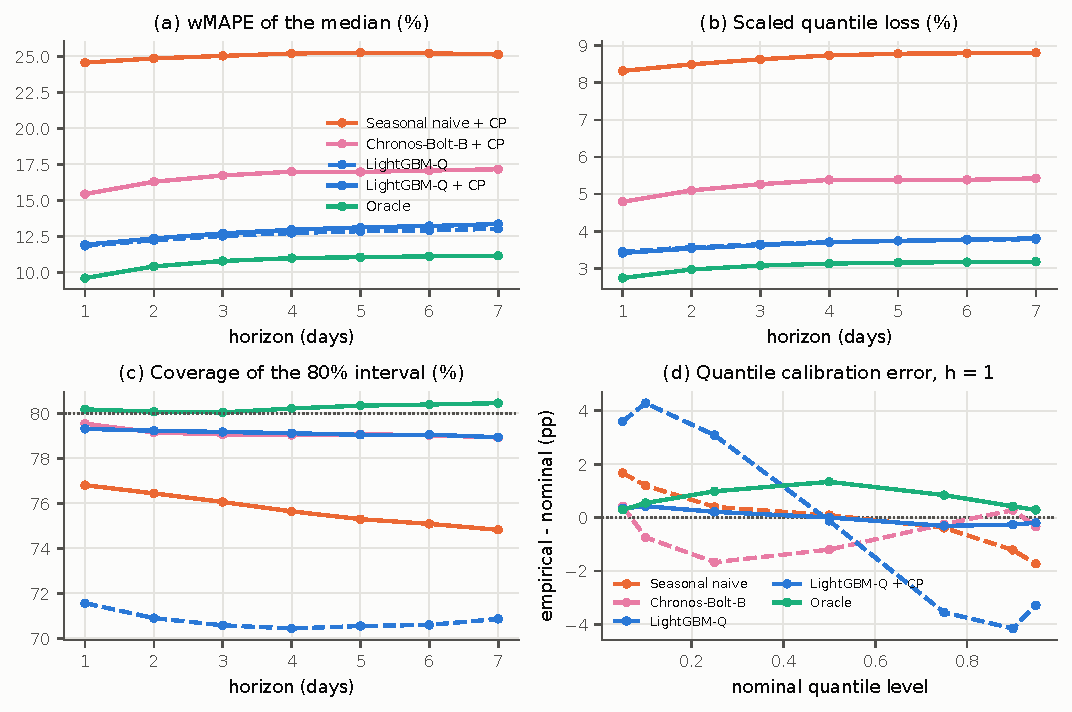
\includegraphics[width=\linewidth]{forecast_accuracy}
  \caption{(a)--(c) Test-year accuracy by horizon. (d) Calibration error of each quantile level at $h=1$ (empirical frequency of $y\le\hat y_a$ minus $a$): raw LightGBM-Q is overconfident in both tails, and conformal calibration removes the error.}
  \label{fig:forecast}
\end{figure}

\Cref{tab:forecast} and \cref{fig:forecast} summarise the test year.
\begin{enumerate}
  \item \textbf{The global LightGBM model halves the error of the seasonal naive benchmark}: day-ahead wMAPE falls from 24.3\% to 11.8\%, and quantile loss from 8.0\% to 3.5\%. It closes about 85\% of the gap between the naive forecast and the oracle (9.6\%). The remaining gap is concentrated around retail events, which occur only twice in the training history.
  \item \textbf{Raw quantile regression is overconfident.} Its 80\% interval covers only 71.6\% of outcomes, a common failure of quantile GBMs on drifting data. Rolling conformal calibration restores nominal coverage (79.3\% and 89.5\%) at a negligible cost in accuracy, by widening the intervals from 31\% to 38\% of demand.
  \item \textbf{The foundation model is a strong zero-shot baseline.} Chronos-Bolt is well calibrated out of the box and, without any training on this data, cuts the naive error by a third (wMAPE 15.4\%). It still trails the covariate-aware LightGBM model by 3.5 points. The reason is visible in \cref{fig:demand}: much of the predictable variance is driven by calendar events, holidays and promotions that a history-only model cannot anticipate. Fine-tuning with covariates is the natural next step (\cref{sec:discussion}).
\end{enumerate}
Feature importance (gain, averaged over the six retrainings) confirms this reading. Weekday (17\%) and holiday status (16\%) dominate, followed by month, the 8-week same-weekday mean, the event-aligned year-over-year ratio and the announced promotion lift (7\% each). These are all information a history-only model does not have.

\subsection{From marginal quantiles to joint scenarios}\label{sec:scenarios}
The planning problem is driven by \emph{aggregates}: the load on a lane is a sum over zones and categories, and the labour of an FC a sum over everything it ships.
How uncertainty adds up therefore matters as much as the marginals.
We generate joint scenarios with a Gaussian copula \citep{nelsen2006}.
\begin{enumerate}
  \item \textbf{Marginals.} The quantile function of every series is interpolated piecewise-linearly in normal-score space $z=\Phi^{-1}(a)$ through the seven forecast quantiles. Beyond the outer levels it is extrapolated linearly, which gives a locally Gaussian tail, and it is truncated at zero.
  \item \textbf{Dependence.} For the last 120 days we compute the probability integral transform (PIT) of each realised value under its own forecast and map it to a normal score. The correlation of these scores across the 260 series, estimated with Ledoit--Wolf shrinkage \citep{ledoit2004}, defines the copula.
  \item \textbf{Sampling.} Draw $\varepsilon\sim\mathcal{N}(0,\hat\Sigma)$ and map each coordinate through its quantile function.
\end{enumerate}
The PIT residuals contain whatever the forecaster failed to predict: national and regional shocks, weather systems, category promotions.
Their correlation is precisely the dependence that remains \emph{conditionally} on the forecast.

\begin{table}[t]
\centering\small
\caption{Quality of joint day-ahead scenarios on the test year (every third day, 1000 scenarios). Energy and variogram scores are computed on the 48 SC$\times$category totals (thousands of units) that load the network; lower is better. Coverage refers to the national daily total.}\label{tab:scenarios}
\begin{tabular}{@{}lrrrrr@{}}\toprule
Scenario generator & Energy & Variogram & \multicolumn{2}{c}{National PI coverage (\%)} & National \\
 & score & score & 50\% & 90\% & CV (\%) \\ \midrule
Seasonal naive + CP, independent & 18.72 & 1068 & 16 & 34 & 5.4 \\
Seasonal naive + CP, copula & 17.53 & 1013 & 60 & 91 & 25.7 \\
LightGBM-Q + CP, independent & 8.23 & 241 & 13 & 30 & 1.9 \\
LightGBM-Q + CP, copula & 8.03 & 242 & 40 & 82 & 6.9 \\
True conditional distribution & 5.88 & 162 & 52 & 88 & 4.8 \\
\bottomrule\end{tabular}

\end{table}

\begin{figure}[t]
  \centering
  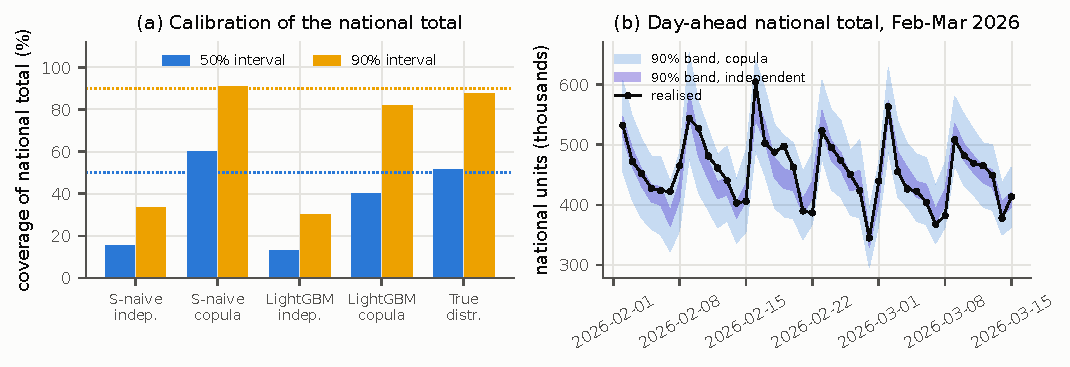
\includegraphics[width=\linewidth]{scenarios}
  \caption{(a) Coverage of the national-total prediction intervals implied by the scenarios. Treating the 260 series as independent makes the national total look three times more certain than it is. (b) Day-ahead 90\% bands for the national total: independent sampling (dark) is far too narrow; the copula (light) contains the realised values.}
  \label{fig:scenarios}
\end{figure}

\Cref{tab:scenarios} and \cref{fig:scenarios} show why this step matters.
With independent sampling the individual series are well calibrated, but the national total is not: its 90\% interval covers the realised value only 30\% of the time, because the coefficient of variation shrinks from 6.9\% to 1.9\% when correlated errors are wrongly assumed to cancel.
The copula restores the coverage to 82\% (50\% interval: 40\%) and improves the energy score on the SC--category totals.
The residual under-coverage reflects a correlation estimated from 120 noisy PIT vectors with shrinkage towards independence, which slightly underestimates the common shock.
The copula intervals are wider than the oracle's (CV 6.9\% vs.\ 4.8\%), as they should be: the forecaster cannot observe the latent states the oracle sees.
